\documentclass[a4paper,12pt]{article}

\usepackage{mystyle}

\graphicspath{ {images/} }


\definecolor{light-cyan}{RGB}{0, 204, 204}
\definecolor{light-purple}{RGB}{138, 43, 226}


\author{Алексеев Василий}
\title{Семинар 1}
\date{1 + 6 сентября 2021}


\begin{document}
  \maketitle
  
  \tableofcontents

  \thispagestyle{empty}
  
  \newpage
  
  \pagenumbering{arabic}


  \section{Матрицы и определители $2$-го и $3$-го порядков}

  Вещественная матрица $A$ размера $m \times n$~---~``таблица'' из чисел $a_{ij} \hm\in \RR$, $i \hm= 1 \ldots m$, $j \hm= 1 \ldots n$:
  \[
    A = \begin{pmatrix}
      a_{11} & a_{12} & \ldots & a_{1n}\\
      a_{21} & a_{22} & \ldots & a_{2n}\\
      \vdots & \vdots & \ddots & \vdots\\
      a_{m1} & a_{m2} & \ldots & a_{mn}
    \end{pmatrix} \in \RR^{m \times n}
  \]
  
  
  \subsection{Операции с матрицами}
  
  \begin{definition}[Сложение матриц]
    Пусть $A, B \in \RR^{n \times n}$.
    Суммой $A \hm+ B$ называется матрица $C \hm\in \RR^{n \times n}$, такая что
    $c_{ij} \hm= a_{ij} + b_{ij}$, $i, j \hm= 1, \ldots, n$.
  \end{definition}
  
  \begin{definition}[Умножение матрицы на число]
    Пусть $A \in \RR^{n \times n}, \alpha \in \RR$.
    Произведением матрицы $A$ на число $\alpha$ называется матрица $C$, такая что
    $c_{ij} \hm= \alpha \cdot a_{ij}$, $i, j \hm= 1, \ldots, n$.
  \end{definition}
  
  \begin{remark}
    Можно проверить, что матрицы $\RR^{n \times n}$ с введённой операцией сложения и умножения на числа из $\RR$ образуют линейное пространство\footnote{\href{https://en.wikipedia.org/wiki/Vector\_space}{wikipedia.org/wiki/Vector\_space}}, то есть операции обладают следующими свойствами:
    \begin{enumerate}
      \item $A + (B + C) = (A + B) + C$, $\forall A, B, C \in \RR^{n \times n}$ (ассоциативность сложения).
      \item $A + B = B + A$, $\forall A, B \in \RR^{n \times n}$ (коммутативность сложения).
      \item $\exists 0_{n\times n} \in \RR^{n \times n}: 0_{n\times n} + A = A$, $\forall A \hm\in \RR^{n \times n}$.
      \item $\forall A \in \RR^{n \times n} \exists {-A} \in \RR^{n \times n}: A + ({-A}) = 0_{n\times n}$.
      \item $\alpha (\beta A) = (\alpha \beta) A$, $\forall \alpha, \beta \in \RR$, $\forall A \hm\in \RR^{n \times n}$ (ассоциативность умножения на скаляр).
      \item $1 \cdot A = A$, $\forall A \in \RR^{n \times n}$.
      \item $(\alpha + \beta) A = \alpha A + \beta A$, $\forall \alpha, \beta \hm\in \RR$, $A \hm\in \RR^{n \times n}$ (дистрибутивность умножения матрицы на число относительно сложения чисел).
      \item $\alpha (A + B) = \alpha A + \alpha B$, $\forall \alpha \hm\in \RR$, $A, B \hm\in \RR^{n \times n}$ (дистрибутивность умножения матрицы на число относительно сложения матриц).
    \end{enumerate}
  \end{remark}
  
  \begin{definition}[Линейная комбинация матриц]
    Линейной комбинацией матриц $A_1, \ldots, A_n$ называется их сумма с некоторыми коэффициентами $\alpha_i \hm\in \RR$:
    \[
      \alpha_1 \cdot A_1 + \ldots + \alpha_n \cdot A_n
    \]
  \end{definition}
  
  
  \begin{problem}[15.2(6)]
    Вычислить линейную комбинацию матриц:
    \[
      2 \begin{pmatrix}
        0 & 0 & 1 & 1 & 1\\
        0 & 1 & 0 & 0 & 1
      \end{pmatrix}
      - \begin{pmatrix}
        1 & 0 & 1 & 1 & 1\\
        0 & 1 & 1 & 1 & 1
      \end{pmatrix} = \?
    \]
  \end{problem}
  
  \begin{solution}
    Вычисляя линейные комбинации соответственных элементов матриц, получаем ответ:
    \[
      \begin{pmatrix}
        -1 & 0 & 1 & 1 & 1\\
        0 & 1 & -1 & -1 & 1
      \end{pmatrix}
    \]
  \end{solution}
  
  
  \begin{definition}[Умножение матриц]
    Пусть $A \hm\in \RR^{m \times p}$, $B \hm\in \RR^{p \times n}$.
    Тогда матрица $C$ называется произведением матриц $A$ и $B$, если
    \[
      \left\{
        \begin{aligned}
          &c_{ij} = \sum_{k = 1}^p a_{ik} b_{kj}\\
          &1 \leq i \leq m\\
          &1 \leq j \leq n
        \end{aligned}
      \right.
    \]
    и обозначается $C \hm= AB$.
  \end{definition}

  \begin{figure}[h]
    \centering
    
    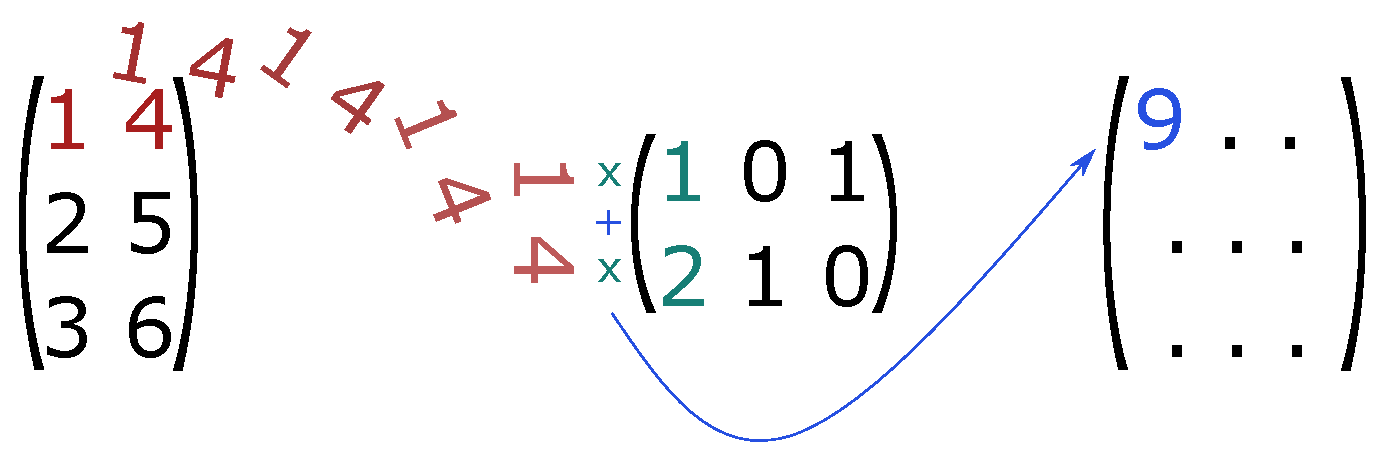
\includegraphics[width=0.5\columnwidth]{matrix-multiplication}
    
    \caption{Иллюстрация умножения матриц.}
    \label{fig:matrix-multiplication}
  \end{figure}
  
  
  \begin{problem}[15.5(12)]
    Вычислить произведение матриц:
    \[
      \begin{pmatrix}
        0         & \ldots & 0         & \lambda_1\\
        0         & \ldots & \lambda_2 & 0\\
        \vdots    & \ddots & \vdots    & \vdots\\
        \lambda_n & \ldots & 0         & 0
      \end{pmatrix}
      \begin{pmatrix}
        \lambda_1 & 0         & \ldots & 0\\
        0         & \lambda_2 & \ldots & 0\\
        \vdots    & \vdots    & \ddots & \vdots\\
        0         & 0         & \ldots & \lambda_n
      \end{pmatrix} = \?
    \]
  \end{problem}
  
  \begin{solution}
    \[
      \begin{pmatrix}
        0         & \ldots & 0         & \lambda_1\\
        0         & \ldots & \lambda_2 & 0\\
        \vdots    & \ddots & \vdots    & \vdots\\
        \lambda_n & \ldots & 0         & 0
      \end{pmatrix}
      \begin{pmatrix}
        \lambda_1 & 0         & \ldots & 0\\
        0         & \lambda_2 & \ldots & 0\\
        \vdots    & \vdots    & \ddots & \vdots\\
        0         & 0         & \ldots & \lambda_n
      \end{pmatrix}
      = \begin{pmatrix}
        0 \cdot \lambda_1 + \ldots + \lambda_1 \cdot 0
          & \ldots
          & 0 + \ldots + \lambda_1 \cdot \lambda_n\\
        \vdots & \ddots & \vdots\\
        \lambda_n \cdot \lambda_1 + \ldots + 0
          & \ldots
          & \lambda_n \cdot 0 + \ldots + 0 \cdot \lambda_n\\
      \end{pmatrix}
      = \begin{pmatrix}
        0                   & \ldots & \lambda_1 \lambda_n\\
        \vdots              & \ddots & \vdots\\
        \lambda_n \lambda_1 & \ldots & 0
      \end{pmatrix}
    \]
  \end{solution}
  
  
  И ещё пара небесполезных концепций из мира матриц.
  
  \begin{definition}[Единичная матрица]
    Матрица $A \in \RR^{n \times n}$ называется единичной, если она нулевая, кроме главной диагонали ($\{a_{ij} \hm\mid i \hm= j\}$), на которой стоят единицы.
    То есть $a_{ij} \hm= 1$ при $i \hm= j$ и $a_{ij} \hm= 0$ при $i \hm{\not=} j$:
    \[
      A = \begin{pmatrix}
        1      & 0      & \ldots & 0       & 0\\
        0      & 1      & \ldots & 0       & 0\\
        \vdots & \vdots & \ddots & \vdots & \vdots\\
        0      & 0      & \ldots & 1      & 0\\
        0      & 0      & \ldots & 0      & 1
      \end{pmatrix}
    \]
    
    Единичная матрица обычно обозначается $E$ или $I$.
  \end{definition}
  
  \begin{definition}[Транспонирование матрицы]
    Пусть $A \in \RR^{n \times n}$.
    Тогда транспонированной по отношению к матрице $A$ матрицей называется такая матрица $С$, что
    $c_{ij} \hm= a_{ji}$.
    Транспонированная матрица обозначается $A^T$.
  \end{definition}
  
  \begin{definition}[След матрицы]
    Следом матрицы $A \in \RR^{n \times n}$ называется сумма элементов, находящихся на главной диагонали $\{a_{ij} \hm\mid i = j, i = 0, \ldots, n\}$:
    \[
      \left\{
        \begin{aligned}
          &\Sp \colon \RR^{n \times n} \to \RR\\
          &\Sp \colon A \mapsto \sum_{i = 1}^n a_{ii}
        \end{aligned}
      \right.
    \]
    У следа есть несколько возможных обозначений.
    Например, можно ещё писать $\Tr A$.
  \end{definition}


  \subsection{Определитель матрицы}
  
  Об определителе можно думать как об особой числовой функции на множестве матриц, обозначаемой $\det$ или $|\cdot|$
  \[
    \det \colon \RR^{n\times n} \to \RR
  \]
  Существует несколько эквивалентных способов определения $\det$: через свойства функции, конкретную формулу вычисления по элементам матрицы \ref{eq:complete-expansion} при произвольном $n$.
  Мы пока опустим строгое определение $\det$ и будем считать, что определитель ``просто есть'', как-то задан.
  И рассмотрим, как его вычислять для квадратных матриц размерностей $2$ и $3$.
  
  \begin{example}
    Определитель второго порядка:
    \[
      \begin{vmatrix}
        a & b\\
        c & d
      \end{vmatrix} = ad - cb
    \]
  \end{example}

  \begin{example}
    Определитель третьего порядка (разложение по первой строке):
    \begin{equation}
    \label{eq:third-order-det-fy-first-line}
    \begin{split}
      &\begin{vmatrix}
        a_1 & b_1 & c_1\\
        a_2 & b_2 & c_2\\
        a_3 & b_3 & c_3
      \end{vmatrix}\\
        =\; &a_1 \cdot \begin{vmatrix}b_2 & c_2\\b_3 & c_3\end{vmatrix}
        - b_1 \cdot \begin{vmatrix}a_2 & c_2\\a_3 & c_3\end{vmatrix}
        + c_1 \cdot \begin{vmatrix}a_2 & b_2\\a_3 & b_3\end{vmatrix}\\
        =\; &a_1 b_2 c_3 - a_1 b_3 c_2 - a_2 b_1 c_3 + a_3 b_1 c_2 + a_2 b_3 c_1 - a_3 b_2 c_1
    \end{split}
    \end{equation}
  \end{example}
  
  Но и при более высоких порядках (четыре и далее) можно использовать тот же алгоритм разложения по первой строке, сводя вычисление определителя порядка $n$ к вычислению нескольких определителей порядка $n \hm- 1$.
  Даже если мы ещё раз посмотрим на определитель второго порядка, то увидим, что он тоже может быть посчитан разложением по первой строке, если положить определитель матрицы размера $1 \hm\times 1$ из одного элемента равным этому самому элементу:
  \[
    \begin{vmatrix}
      a & b\\
      c & d
    \end{vmatrix}
    = a \cdot |d| - b \cdot |c|
    \xrightarrow{|x| \equiv x} ad - cb
  \]
  
  Таким образом, мы уже фактически пришли к следующему варианту определить функцию $\det$:
  
  \begin{definition}[Определитель (рекурсивный вариант определения)]
    Положим определитель матрицы из одного элемента равным этому самому элементу
    \[
      \det \begin{pmatrix}a\end{pmatrix} \equiv a
    \]
    Пусть $d_{ij}$~---~определитель подматрицы $D_{ij}$ матрицы $A \in \RR^{n \times n}$, которая получается при вычёркивании $i$-ой строки и $j$-го столбца.
    Тогда
    \[
      \det(A) = \sum\limits_{j = 1}^n a_{ij} (-1)^{i + j} d_{ij}
    \]
    где $i$~---~любая строка матрицы $A$ (не важно, какая~---~значение функции $\det$ не изменится).
  \end{definition}
  
  \begin{problem}[14.7(3)]
    \[
      \begin{vmatrix}
        1 & 2 & 2\\
        2 & 1 & -2\\
        2 & -2 & 1
      \end{vmatrix} = \?
    \]
  \end{problem}
  
  \begin{solution}
    \[
      \begin{vmatrix}
        1 & 2 & 2\\
        2 & 1 & -2\\
        2 & -2 & 1
      \end{vmatrix}
      = 1 \cdot \Bigl(1 \cdot 1 - (-2) \cdot (-2)\Bigr)
        \textcolor{light-cyan}{-} 2 \cdot \Bigl(2 \cdot 1 - 2 \cdot (-2)\Bigr)
        + 2 \cdot \Bigl(2 \cdot (-2) - 2 \cdot 1\Bigr)
      = -3 - 12 - 12
      = -27
    \]
  \end{solution}
  
  
  \section{Системы линейныx уравнений. Правило Крамера}
  
  Система $m$ линейных уравнений с $n$ неизвестными:
  \[
    \renewcommand{\arraycolsep}{2pt}
    \left\{
      \begin{array}{lcl}
        a_{11} x_1 + \ldots + a_{1n} x_n & = & b_1\\
        \hdotsfor{3}\\
        a_{m1} x_1 + \ldots + a_{mn} x_n & = & b_m
      \end{array}
    \right.
  \]
  
  В матричном виде:
  \[
    \begin{pmatrix}
      a_{11} & \ldots & a_{1n}\\
      \vdots & \ddots & \vdots\\
      a_{m1} & \ldots & a_{mn}
    \end{pmatrix}
    \begin{pmatrix}
      x_1\\
      \vdots\\
      x_n
    \end{pmatrix}
    =
    \begin{pmatrix}
      b_1\\
      \vdots\\
      b_m
    \end{pmatrix}
  \]
  
  Или так:
  \[
    A_{m \times n} \bds x_{n \times 1} = \bds b_{m \times 1}
  \]
  
  \begin{definition}[Решение системы]
    \[
      \{\bds x \in \RR^n \mid A \bds x = \bds b\}
    \]
  \end{definition}
  
  \begin{definition}
    Система называется совместной, если она имеет хотя бы одно решение, и несовместной, если у неё нет решений.
  \end{definition}
  
  \begin{definition}
    Говорят, что система $B$ следует из системы $A$, если множество решений $B$ содержит множество решений $A$ (\ref{fig:a-and-b-sets}).
  \end{definition}
  
  \begin{figure}[h]
    \centering
    
    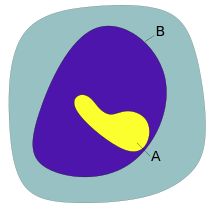
\includegraphics[width=0.5\columnwidth]{a-and-b-sets}
    
    \caption{Множество решений $A$ содержится во множестве решений $B$.}
    \label{fig:a-and-b-sets}
  \end{figure}
  
  \begin{theorem}
    Пусть число уравнений в системе $m$ равно числу неизвестных $n$.
    Тогда если $\det A \hm{\not=} 0$, то система $A \bds x \hm= \bds b$ имеет решение, и притом только одно.
  \end{theorem}
  
  \begin{theorem}[Правило Крамера]
    Пусть число уравнений в системе $m$ равно числу неизвестных $n$.
    Тогда если $\det A \hm{\not=} 0$, то
    \[
      \left\{
        \begin{aligned}
          &x_i = \frac{\Delta_i}{\Delta}\\
          &\Delta \equiv \det A\\
          &\Delta_i \equiv \det (\bds a_1, \ldots, \bds a_{i - 1}, \bds b, \bds a_{i + 1}, \ldots, \bds a_n)
        \end{aligned}
      \right.
    \]
  \end{theorem}
  
  
  \begin{example}
    Если определитель матрицы системы равен нулю, то решений может как не быть вообще, так и быть бесконечно много.
    Например:
    \[
      \left\{
        \begin{aligned}
          &x + y = 2\\
          &x + y = -1
        \end{aligned}
      \right.
      \quad \left\{
        \begin{aligned}
          &x + y = 2\\
          &x + y = 2
        \end{aligned}
      \right.
    \]
  \end{example}
  
  
  \begin{problem}[17.1(2)]
    Решить систему:
    \[
      \left\{
        \begin{aligned}
          &3x + 5y = 2\\
          &5x + 9y = 4
        \end{aligned}
      \right.
    \]
  \end{problem}
  
  \begin{solution}
    Перепишем систему в матричном виде:
    \[
      \left\{
        \begin{aligned}
          &A \bds x = \bds b\\
          &A = \begin{pmatrix}
            3 & 5\\
            5 & 9
          \end{pmatrix}\\
          &\bds b = \begin{pmatrix}
            2 & 4
          \end{pmatrix}^T
        \end{aligned}
      \right.
    \]
    
    Расширенная матрица системы: $(A | \bds b)$.
    
    Матрица $A$ квадратная.
    Её определитель $|A| = 2$ отличен от нуля.
    Поэтому решение системы существует и единственно.
    И его можно найти по формулам:
    
    \[
      \Delta = \det A = \det \begin{pmatrix}
        3 & 5\\
        5 & 9
      \end{pmatrix} = 2
    \]
    \[
      \Delta_x = \det \begin{pmatrix}
        2 & 5\\
        4 & 9
      \end{pmatrix} = -2 \Rightarrow x = \frac{\Delta_x}{\Delta} = \frac{-2}{2} = -1
    \]
    \[
      \Delta_y = \det \begin{pmatrix}
        3 & 2\\
        5 & 4
      \end{pmatrix} = 2 \Rightarrow y = \frac{\Delta_y}{\Delta} = \frac{2}{2} = 1
    \]
    
    И решение:
    \[
      \bds x = \begin{pmatrix}
        x & y
      \end{pmatrix}^T = \begin{pmatrix}
        -1 & 1
      \end{pmatrix}^T
    \]
  \end{solution}
  
  
  \newpage
  
  
  \section{Дополнение}
  
  В дополнении приведём ещё один способ считать определитель третьего порядка.
  Отметим ``роль'' главной диагонали.
  И далее приведём ещё несколько равносильных способов задать определитель (без доказательства равносильности), отметим пару свойств определителя.
  
  
  \subsection{Правило треугольника}
  
  (Как было замечено на семинаре) при подсчёте определителя третьего порядка ещё можно пользоваться т.н. ``правилом треугольника'' (\ref{fig:triangle-rule}).
  
  \begin{figure}[h]
    \centering
    
    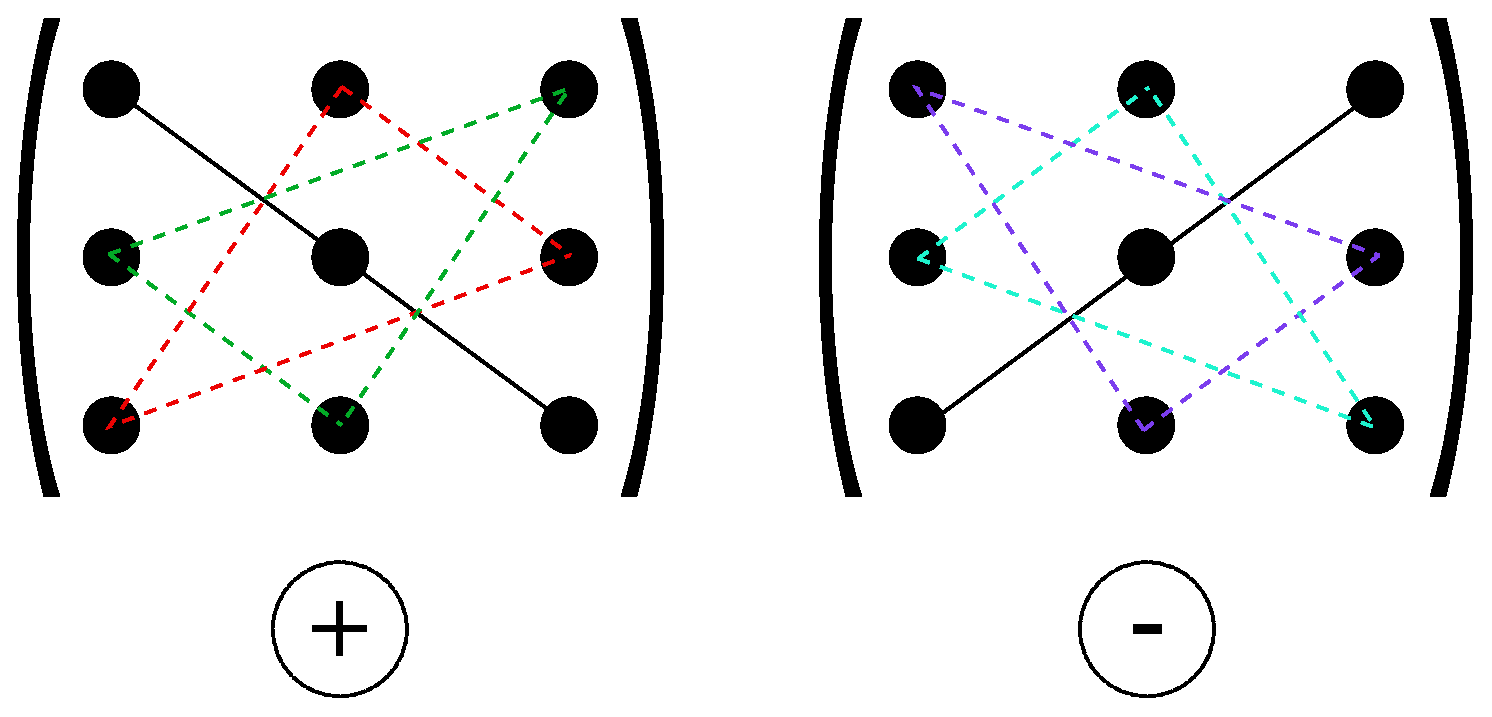
\includegraphics[width=0.6\columnwidth]{triangle-rule}
    
    \caption{Правило треугольника для вычисления определителя третьего порядка.}
    \label{fig:triangle-rule}
  \end{figure}
  
  Если сложить все тройки, сначала с плюсом, потом с минусом, то получаем (первая тройка в каждом ``блоке''~---~диагональные элементы):
  \begin{equation*}
    \begin{vmatrix}
      a_1 & b_1 & c_1\\
      a_2 & b_2 & c_2\\
      a_3 & b_3 & c_3
    \end{vmatrix}
      = a_1 b_2 c_3 + a_3 b_1 c_2 + a_2 b_3 c_1 - a_3 b_2 c_1 - a_1 b_3 c_2 - a_2 b_1 c_3
  \end{equation*}
  
  Что совпадает, с точностью до перестановки троек, с формулой вычисления по первой строке (\ref{eq:third-order-det-fy-first-line}).
  
  Ещё есть (возможно, не такое красивое, как с треугольниками) правило Саррюса (\ref{fig:determinant-sarrus}).
  
  \begin{figure}[h]
    \centering
    
    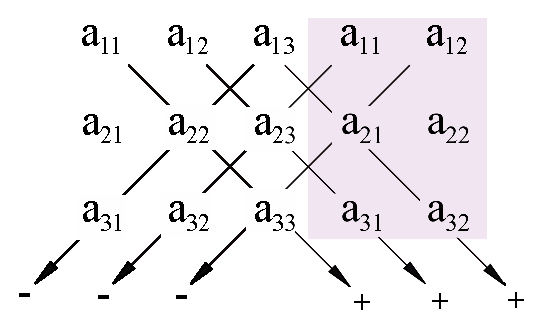
\includegraphics[width=0.5\columnwidth]{determinant-sarrus}
    
    \caption{Правило Саррюса для вычисления определителя третьего порядка (картинка взята с русской страницы \href{https://upload.wikimedia.org/wikipedia/commons/1/17/Determinant-sarrus.svg}{Википедии}).}
    \label{fig:determinant-sarrus}
  \end{figure}
  
  
  \subsection{Диагональные дела}
  
  Главная диагональ, как для квадратных, так и для прямоугольных матриц, определяется как множество элементов матрицы с одинаковыми индексами: $\bigl\{a_{ij} \hm\mid i \hm= j,\ i \hm\in \{1, \ldots, m\},\ j \hm\in \{1, \ldots, n\}\bigr\}$.
  
  Где в мире прямоугольных матриц может встречаться понятие главной диагонали?
  О транспонировании можно думать, как об отражении матрицы относительно главной диагонали (\ref{fig:main-diagonal}).
  
  \begin{figure}[h]
    \centering
    
    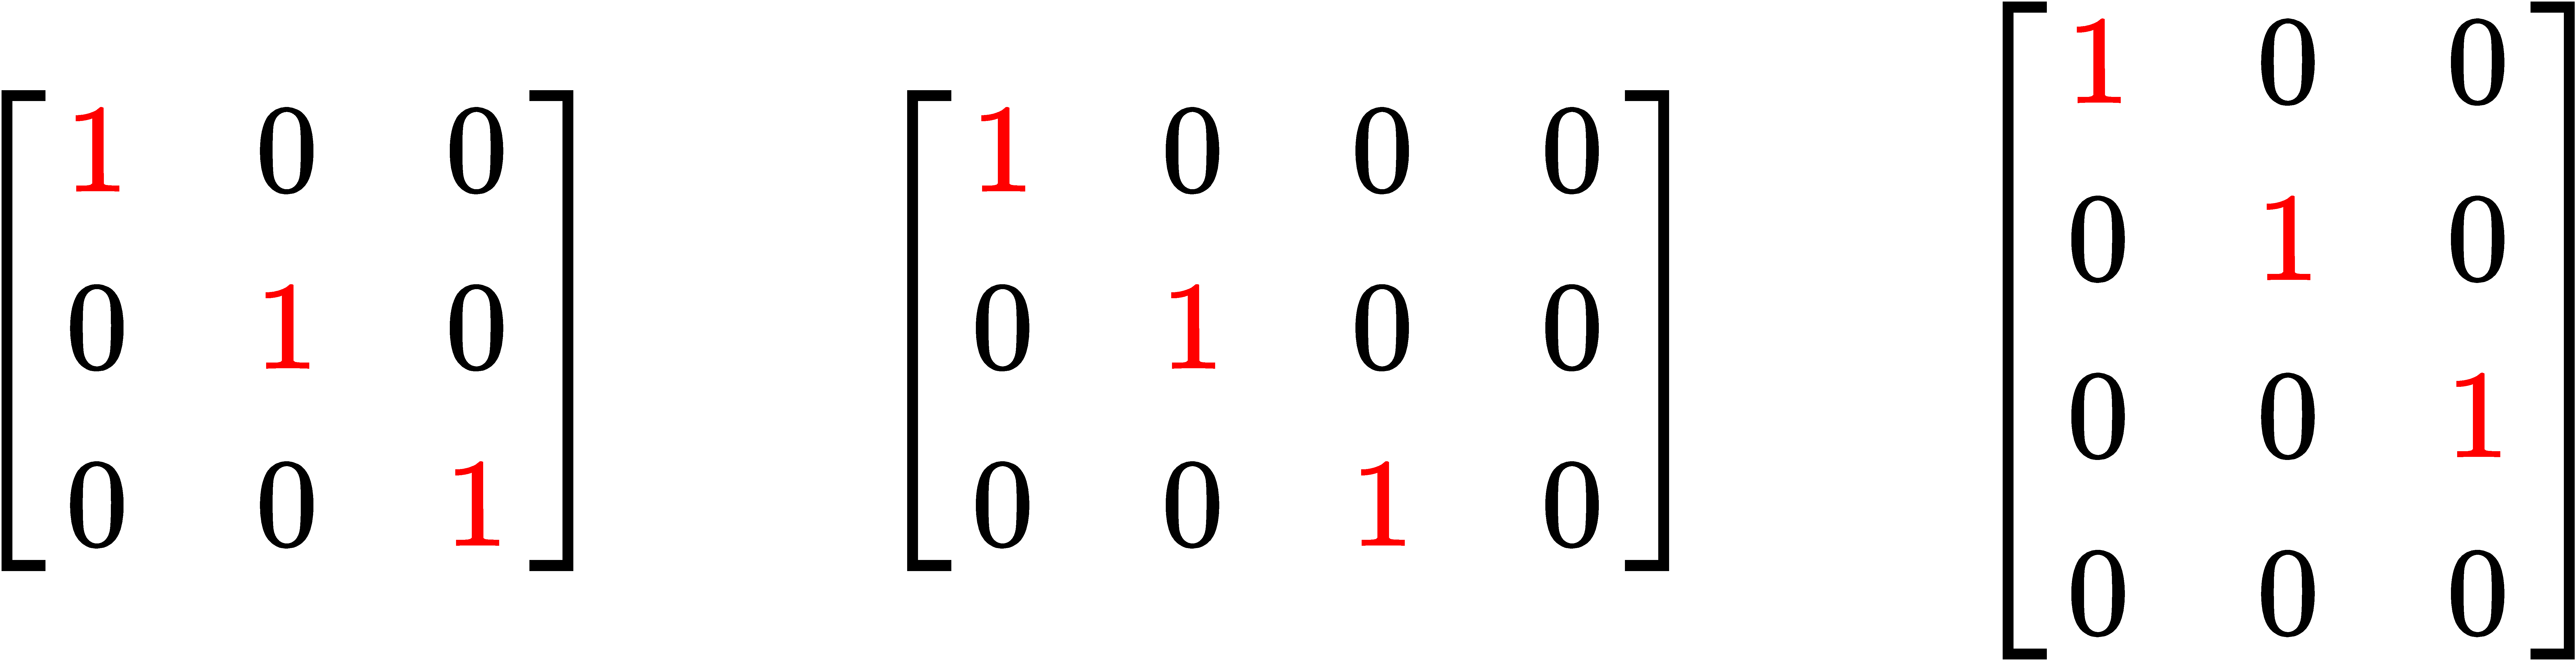
\includegraphics[width=0.5\columnwidth]{main-diagonal}
    
    \caption{Главная диагональ прямоугольной матрицы (картинка с \href{https://en.wikipedia.org/wiki/Main\_diagonal}{en.wikipedia.org/wiki/Main\_diagonal}).}
    \label{fig:main-diagonal}
  \end{figure}
  
  Также известно, например, что любую прямоугольную матрицу можно представить в виде произведения трёх матриц с определёнными свойствами (SVD разложение).
  Не обращая внимание на левый и правый множители, заметим лишь, что у матрицы-множителя посередине ненулевые элементы в SVD разложении могут стоять только на главной диагонали (\ref{fig:svd_reduced}).
  
  \begin{figure}[h]
    \centering
    
    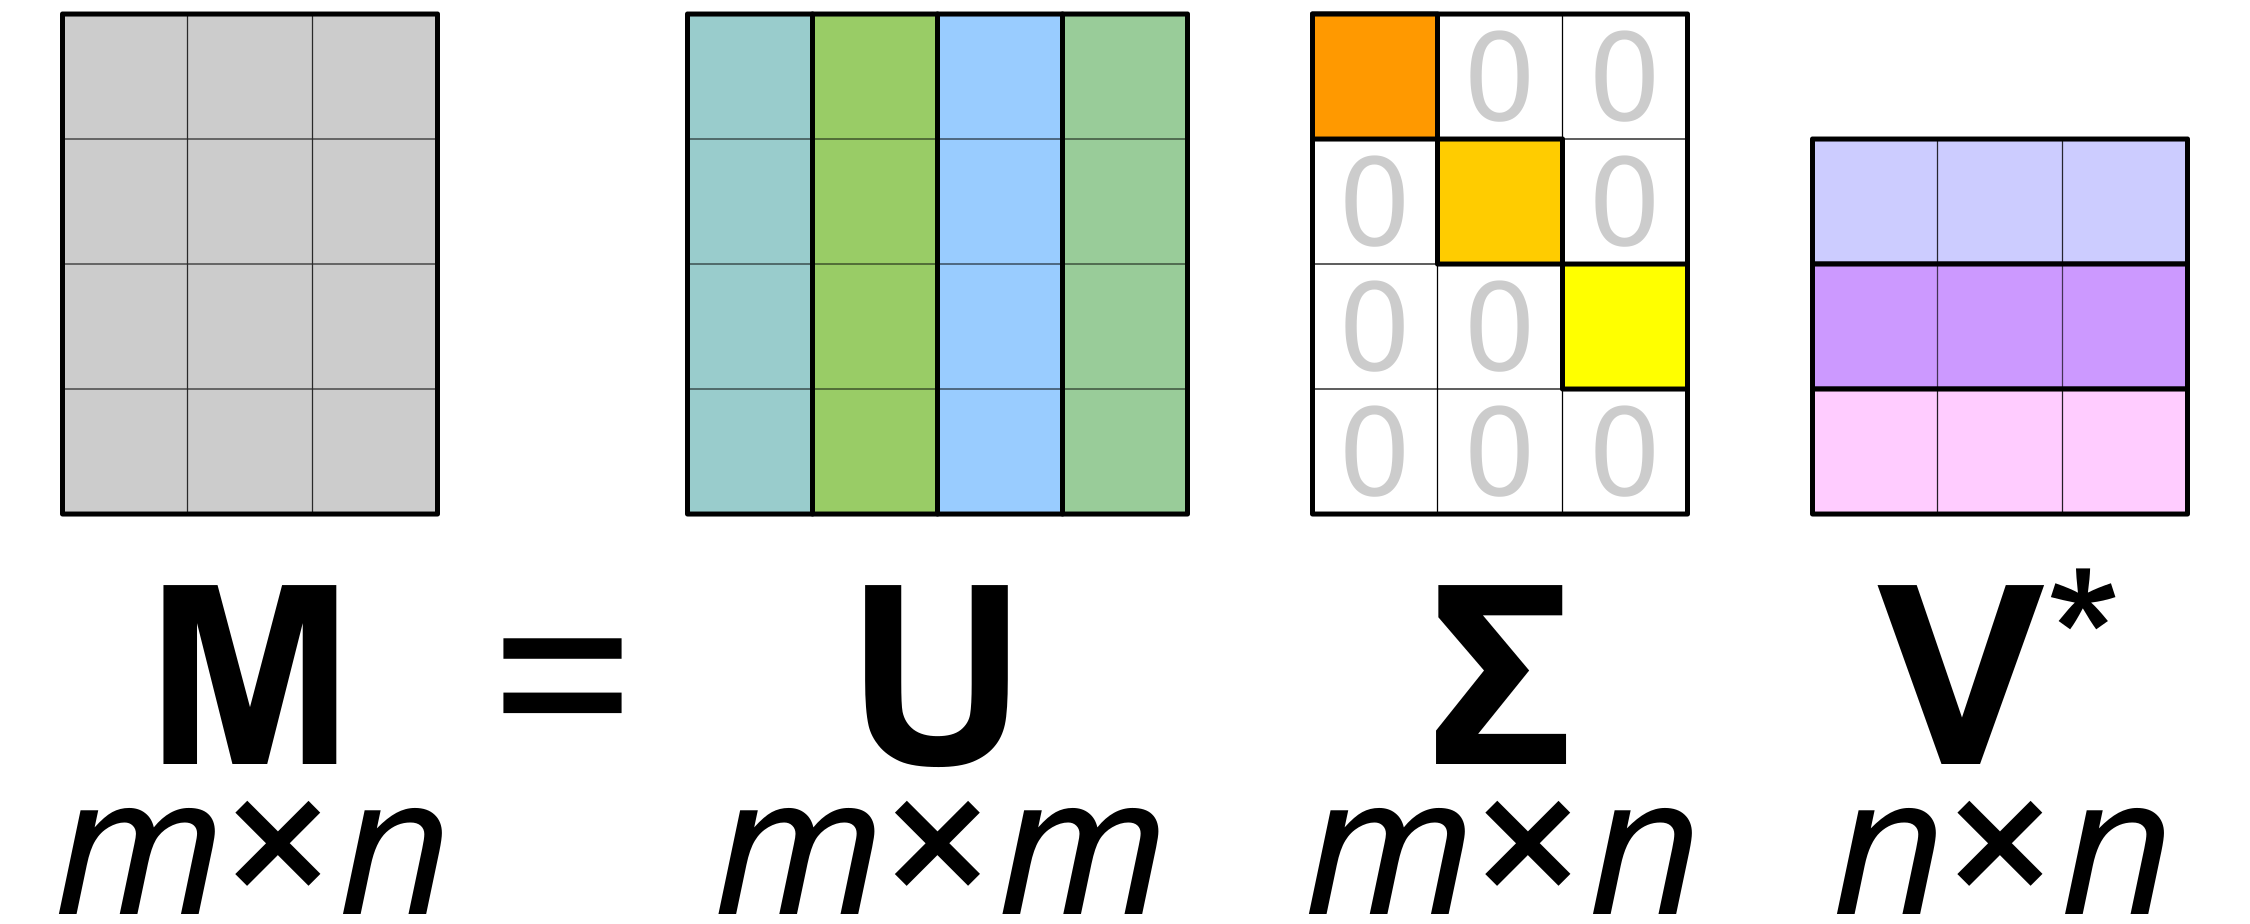
\includegraphics[width=0.5\columnwidth]{svd_reduced}  % TODO: make svg for this pic
    
    \caption{SVD разложение прямоугольной матрицы (картинка с \href{https://commons.wikimedia.org/wiki/File:Singular\_value\_decomposition_visualisation.svg}{en.wikipedia.org/wiki/Singular\_value\_decomposition}).}
    \label{fig:svd_reduced}
  \end{figure}

  Побочная же диагональ вводится только для квадратных матриц $A \hm\in \RR^{n \hm\times n}$ как множество следующих элементов: $\bigl\{a_{ij} \hm\mid i \hm+ j \hm= n \hm+ 1,\ i \hm\in \{1, \ldots, n\},\ j \hm\in \{1, \ldots, n\}\bigr\}$ (\ref{fig:secondary-diagonal}).
  
  \begin{figure}[h]
    \centering
    
    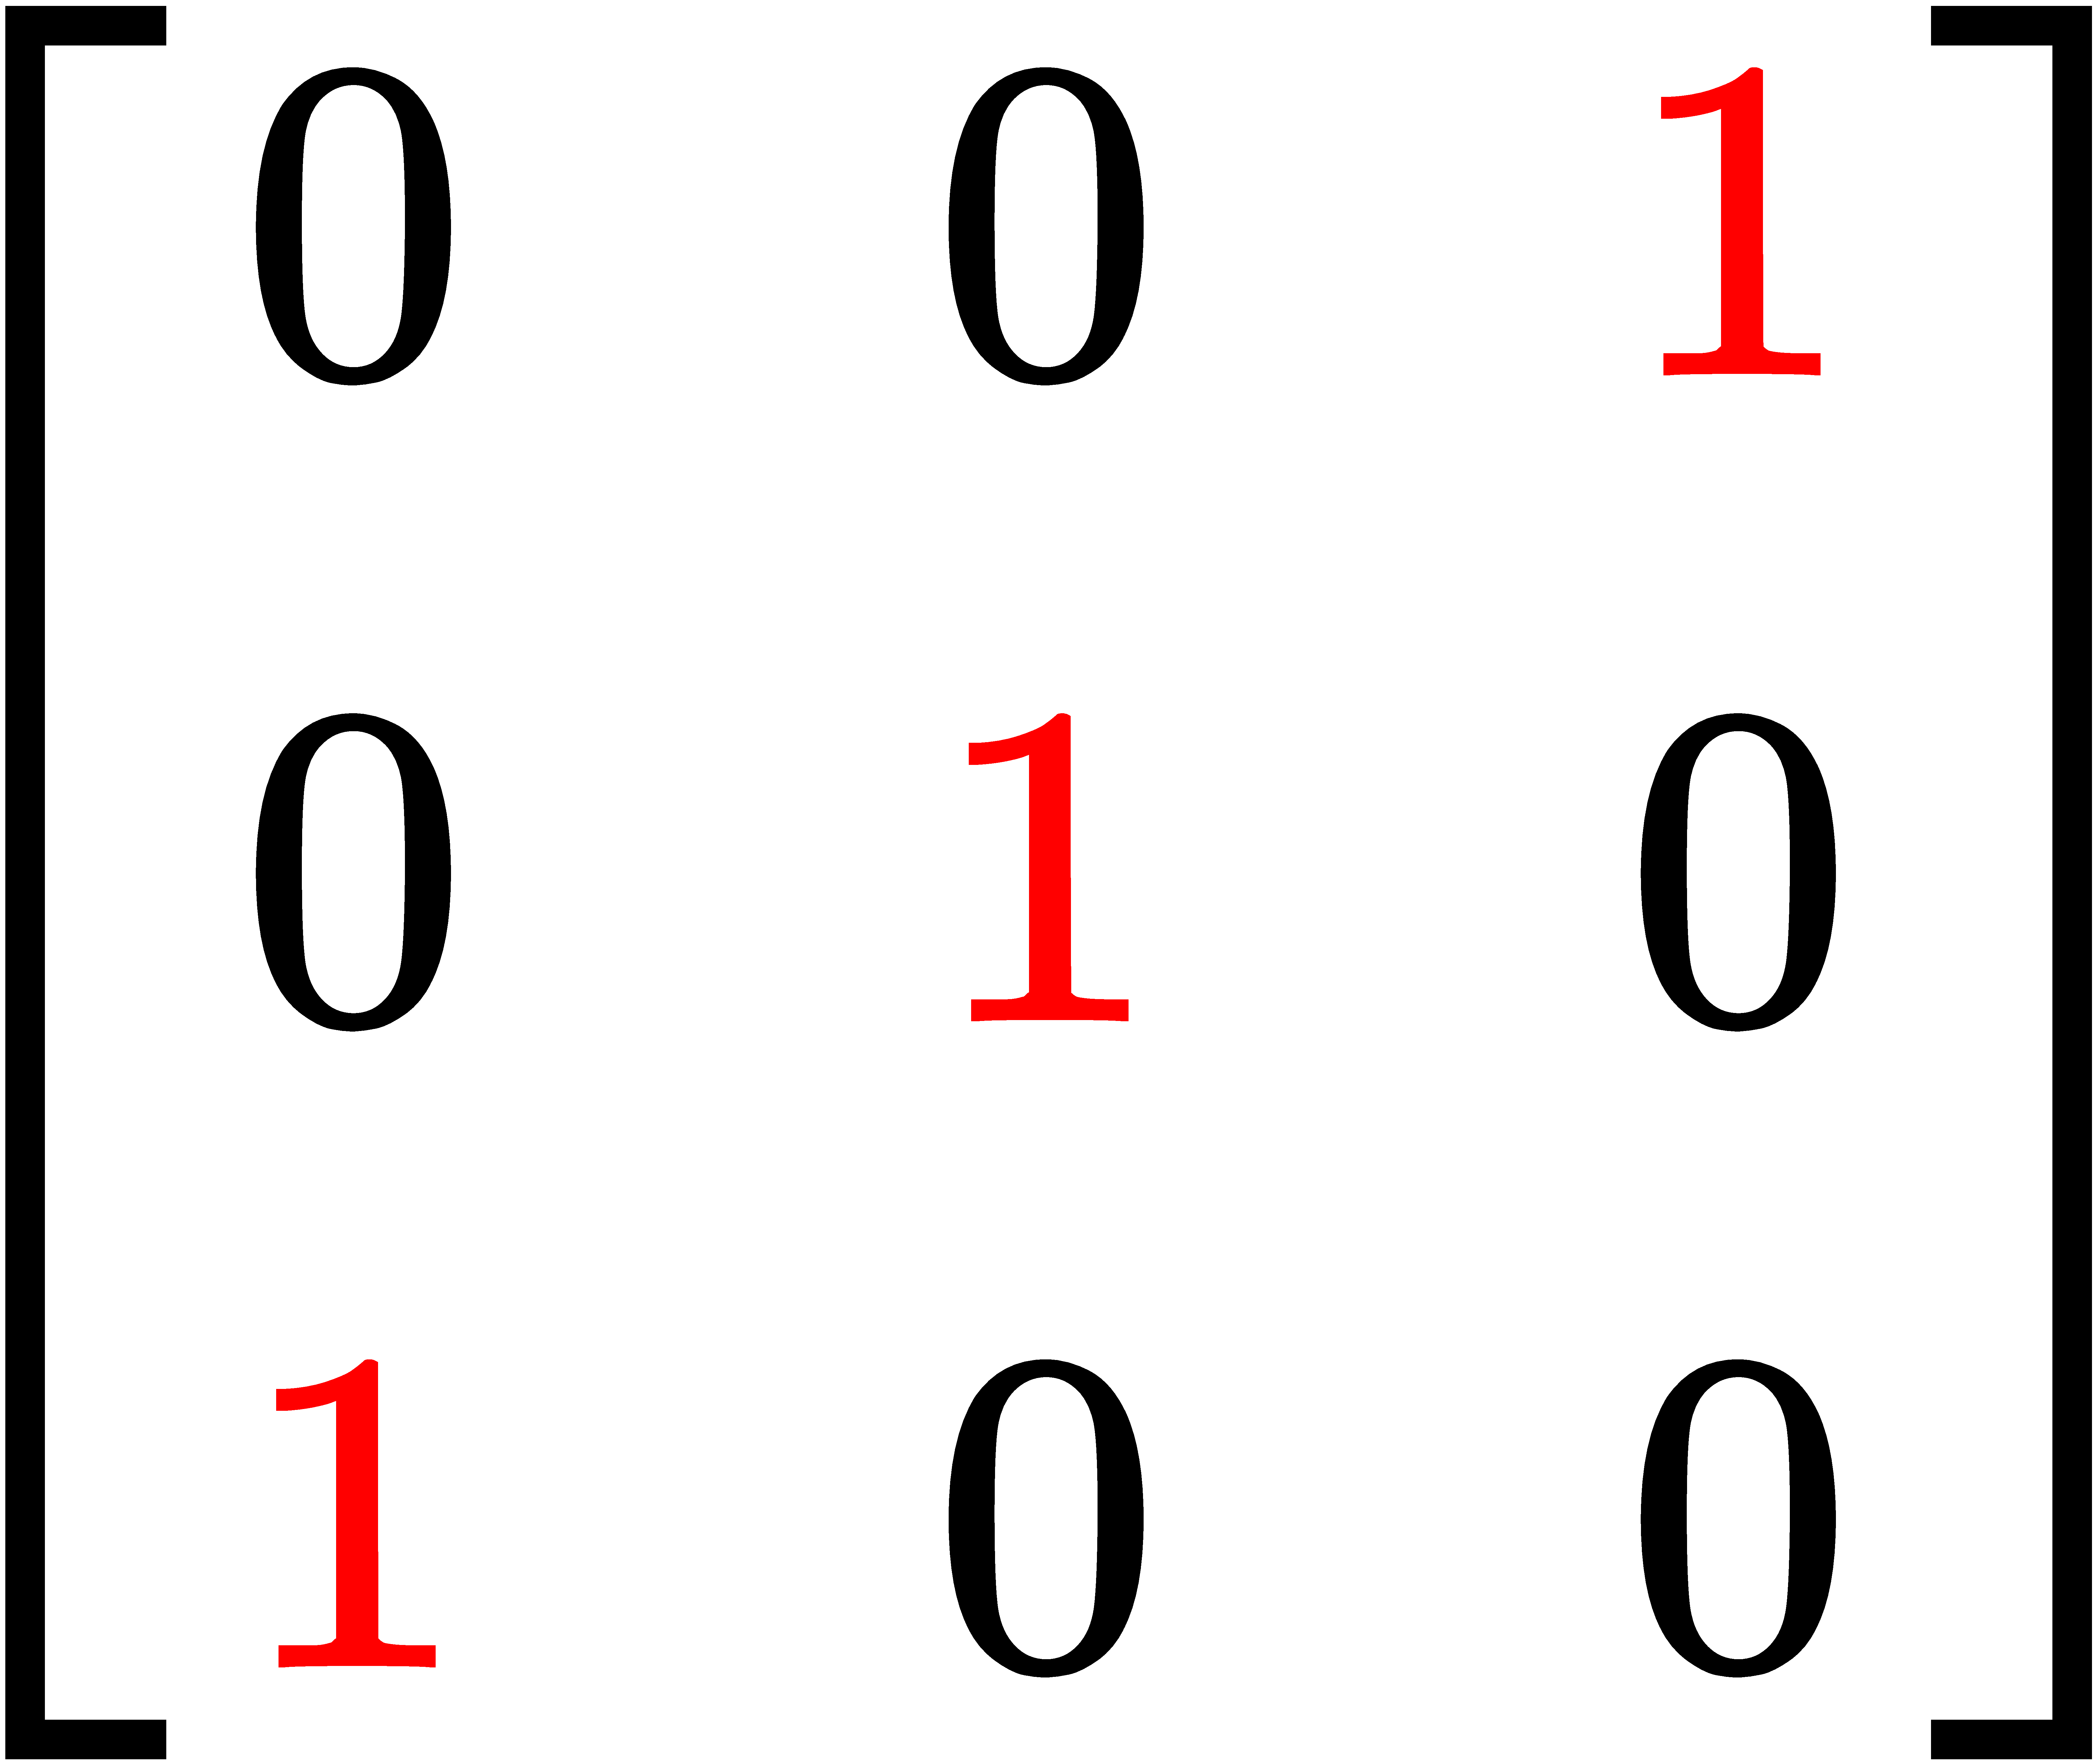
\includegraphics[width=0.11\columnwidth]{secondary-diagonal}  % TODO: make size of one matrix the same as for the pic with main diagonal
    
    \caption{Побочная диагональ квадратной матрицы (картинка с \href{https://en.wikipedia.org/wiki/Main\_diagonal}{en.wikipedia.org/wiki/Main\_diagonal}).}
    \label{fig:secondary-diagonal}
  \end{figure}
  
  
  \subsection{Задание определителя с помощью формулы}
  
  \begin{theorem}[Формула полного разложения определителя]\label{theor:complete-expansion}
    Пусть $A \in \RR^{n \times n}$.
    Тогда определитель $\det A$ матрицы равен
    \begin{equation}
      \label{eq:complete-expansion}
      \det A = \sum_{(i_1, \ldots, i_n)} (-1)^{N(i_1, \ldots, i_n)} a_{1 i_1} \ldots a_{n i_n}
    \end{equation}
    где $N(i_1, \ldots, i_n)$~---~число нарушений порядка в перестановке чисел $i_1, \ldots, i_n$\footnote{Нарушение порядка~---~когда правее большего элемента стоит меньший элемент: $i_k > i_s$, но $k < s$.}.
    Сумма в формуле берётся по всем перестановкам чисел $1, \ldots, n$\footnote{Например, перестановки чисел $1, 2, 3$: $(1, 2, 3), (1, 3, 2), (2, 1, 3), (2, 3, 1), (3, 1, 2), (3, 2, 1)$.}.
  \end{theorem}
  
  \begin{example}
    Вспомним формулу вычисления определителя для матрицы размера $3$:
    \begin{equation*}
      \begin{vmatrix}
        a_1 & b_1 & c_1\\
        a_2 & b_2 & c_2\\
        a_3 & b_3 & c_3
      \end{vmatrix}
        = a_1 b_2 c_3 - a_1 b_3 c_2 - a_2 b_1 c_3 + a_3 b_1 c_2 + a_2 b_3 c_1 - a_3 b_2 c_1
    \end{equation*}
    
    Элементы в каждом слагаемом упорядочены по номеру столбца.
    Поэтому посмотрим на число беспорядков по строкам (неважно, как считать беспорядки, по строкам или по столбцам, потому что $\det A \hm= \det A^T$).
    В первом слагаемом: $N(1, 2, 3) \hm= 0$.
    Во втором: $N(1, 3, 2) \hm= 1$ (тройка и двойка).
    В третьем: $N(2, 1, 3) \hm= 1$ (двойка и единица).
    В четвёртом: $N(3, 1, 2) \hm= 2$ (два беспорядка с тройкой и единицей и тройкой и двойкой).
    В пятом: $N(2, 3, 1) \hm= 1 \hm+ 1 \hm= 2$ (для двойки и единицы и для тройки и единицы).
    В шестом: $N(3, 2, 1) \hm= 2 \hm+ 1 \hm= 3$ (тройка-двойка, тройка-единица, двойка-единица).
  \end{example}
  
  
  \subsection{Свойства определителя}
  
  \begin{theorem}
    Некоторые свойства определителя (матрицы в формулах ниже представляются столбцами $\bds a_i \hm\in \RR^n$):
    \begin{enumerate}
      \item Линейность по столбцу (строке)~---~полилинейность:
        \begin{equation}\label{eq:poly-linearity}
          \left\{
            \begin{aligned}
              &\det (\bds a_1, \ldots, \underbrace{\bds p + \bds q}_{\bds a_i}, \ldots, \bds a_n)
                = \det (\bds a_1, \ldots, \bds p, \ldots, \bds a_n)
                + \det (\bds a_1, \ldots, \bds q, \ldots, \bds a_n)\\
              &\det (\bds a_1, \ldots, \underbrace{\alpha \bds p}_{\bds a_i}, \ldots, \bds a_n)
                = \alpha \det (\bds a_1, \ldots, \bds p, \ldots, \bds a_n)
            \end{aligned}
          \right.
        \end{equation}
      \item При перестановке двух столбцов (строк) матрицы её определитель меняет знак (кососимметричность, антисимметричность по столбцам/строкам):
        \begin{equation}\label{eq:row-swap}
          \det (\bds a_1, \ldots, \bds a_{\textcolor{light-cyan}{i}}, \ldots, \bds a_{\textcolor{light-purple}{j}}, \ldots, \bds a_n)
          = -\det (\bds a_1, \ldots, \bds a_{\textcolor{light-purple}{j}}, \ldots, \bds a_{\textcolor{light-cyan}{i}}, \ldots, \bds a_n)
        \end{equation}
      \item Если два столбца (две строки) матрицы совпадают, то её определитель равен нулю:
        \begin{equation}\label{eq:same-rows}
          \det (\bds a_1, \ldots, \bds p, \ldots, \bds p, \ldots, \bds a_n) = 0
        \end{equation}
    \end{enumerate}
  \end{theorem}
  
  Свойства можно доказать как следствия теоремы \ref{theor:complete-expansion}.
  
  И ещё пара более частных утверждений, которые следуют/являются подслучаями свойств выше:
  \begin{itemize}
    \item Общий множитель элементов строки (столбца) можно выносить за знак определителя:
      \[
        \det (\bds a_1, \ldots, \alpha \bds p, \ldots, \bds a_n)
          = \alpha \cdot \det (\bds a_1, \ldots, \bds p, \ldots, \bds a_n)
      \]
    \item К любой строке (столбцу) матрицы можно прибавлять линейную комбинацию других строк (столбцов)~---~определитель при этом не изменится:
      \[
        \det (\bds a_1, \ldots, \bds a_i, \ldots, \bds a_n)
          = \det (\bds a_1, \ldots, \sum_{\substack{1 \leq j \leq n\\j \not= i}} \alpha_j \bds a_j + \bds a_i, \ldots, \bds a_n)
      \]
    \item При вычислении определителя матрицы вида $\alpha A$ скаляр $\alpha$ можно выносить за знак $\det$ следующим образом:
      \[
        \det \alpha A = \alpha^n \det A
      \]
  \end{itemize}
  
  И посмотрим, чему равен определитель нескольких специального вида матриц.
  
  \begin{example}
    Определитель единичной матрицы:
    \[
      \det E = 1^n = 1
    \]
  \end{example}
  
  \begin{definition}[Вырожденная матрица\footnote{Определение вырожденной матрицы можно вводить по-разному. Ещё возможный вариант: квадратная матрица называется вырожденной, если её строки $\{\bds a_i\}_{i=1}^n$ линейно зависимы. Строки линейно зависимы~---~когда существует нетривиальная линейная комбинация строк, которая даёт нулевую строку: $\sum_{i=1}^n \alpha_i \bds a_i \hm= \bds 0$, $\sum_{i=1}^n \alpha_i^2 \hm > 0$.}]
    Матрица $A$ называется вырожденной, если $\det A \hm= 0$.
    В противном случае матрица $A$ называется невырожденной.
  \end{definition}
  
  \begin{theorem}
    Определитель транспонированной матрицы
    \[
      \det A^T = \det A
    \]
  \end{theorem}
  
  \begin{theorem}
    Определитель произведения двух квадратных матриц:
    \[
      \det (AB) = \det A \cdot \det B
    \]
  \end{theorem}
  
  \begin{theorem}
    Определитель матрицы, обратной к \emph{невырожденной} матрице
    \[
      \det A^{-1} = \bigl(\det A\bigl)^{-1}
    \]
  \end{theorem}
  

  \subsection{Задание определителя через свойства}
  
  Как отмечалось выше, существует несколько эквивалентных определений $\det$.
  Один из способов~---~с помощью формулы (\ref{eq:complete-expansion}).
  Приведём далее ещё пару, основанных на перечислении свойств, которыми должна обладать функция $\det$.
  
  \begin{definition}[Вариант $1$\footnote{Беклемишев~Д.~В. <<Курс аналитической геометрии и линейной алгебры>>}]
    Функция $f \colon \RR^{n \times n} \to \RR$ называется определителем (детерминантом) и обозначается $\det$, если
    \begin{itemize}
      \item Функция $f$ является линейным однородным многочленом от элементов любой строки:
      \[
        \left\{
          \begin{aligned}
            &f(A) = h_1 a_{i1} + \ldots + h_n a_{in}\\
            &1 \leq i \leq n\\
            &h_j = h_j(a_1, \ldots, a_{i-1}, a_{i+1}, \ldots, a_{n}),\ 1 \leq j \leq n
          \end{aligned}
        \right.
      \]
      то есть коэффициенты в разложении по элементам строки не зависят от этой самой строки.
      
      \item Значение $f$ на вырожденной матрице\footnote{У которой строки линейно зависимы} равно нулю $0$.
      \item Значение $f$ на единичной матрице $E_{n \times n}$ равно единице $1$.
    \end{itemize}
  \end{definition}
  
  \begin{definition}[Вариант $2$\footnote{\href{https://en.wikipedia.org/wiki/Determinant\#Definition}{https://en.wikipedia.org/wiki/Determinant}}]
    Функция $f \colon \RR^{n \times n} \to \RR$ называется определителем (детерминантом) и обозначается $\det$, если
    \begin{itemize}
      \item Функция $f$ полилинейна по строкам матрицы $A \in \RR^{n \times n}$ (\ref{eq:poly-linearity}).
      \item Функция $f$ кососимметрична по строкам матрицы $A$ (\ref{eq:row-swap}).
      \item Значение $f$ на единичной матрице $E_{n \times n}$ равно единице $1$.
    \end{itemize}
  \end{definition}
  
  \begin{definition}[Вариант $3$\footnote{Hans Schneider, George Phillip Barker. <<Matrices and Linear Algebra>>}]
    Функция $f \colon \RR^{n \times n} \to \RR$ называется определителем (детерминантом) и обозначается $\det$, если
    \begin{itemize}
      \item Функция $f$ полилинейна по строкам матрицы $A \in \RR^{n \times n}$ (\ref{eq:poly-linearity}).
      \item Значение $f$ на матрице с двумя одинаковыми строками равно нулю $0$ (\ref{eq:same-rows}).
      \item Значение $f$ на единичной матрице $E_{n \times n}$ равно единице $1$.
    \end{itemize}
  \end{definition}
\end{document}